\chapter{Les propietats i el comportament dels gasos}

L'estudi dels gasos és fonamental per a comprendre el comportament de la matèria en estat gasós. Aquests conceptes són claus tant en la química moderna com en l'aplicació industrial. Les lleis dels gasos proporcionen una base per descriure el comportament macroscòpic dels gasos en funció de la temperatura, el volum i la pressió.



\section{Les lleis dels gasos}
En general, el volum d'un gas està determinat per la seva temperatura i la pressió que suporta. Existeix una relació matemàtica entre aquests paràmetres, que s'expressa com l'\textbf{equació d'estat}:
\begin{equation}
V = V(T, P, n),
\end{equation}
on $V$ és el volum, $T$ és la temperatura, $P$ la pressió, i $n$ el nombre de mols del material. Es tracta d'una equació que pot ser molt complexa i específica per a líquids i sòlids, però en el cas dels gasos tots ells tenen un comportament molt similar. Això és degut a que en l'estat gas, les molècules són mes independents entre elles i, per tant, la seva naturalesa molecular no afecta substancialment al comportament del tot.

\begin{mybox}[title=De partícules i mols de partícules]
    El mol és la unitat bàsica del Sistema Internacional per mesurar la quantitat de substància, i s'utilitza per comptar partícules com àtoms, molècules o ions. Un mol conté exactament \(6,022 \times 10^{23}\) entitats elementals, un valor conegut com el nombre d'Avogadro. Aquesta constant permet connectar les dimensions microscòpiques (com la massa i el nombre de partícules) amb mesures macroscòpiques utilitzades en els experiments químics. Per exemple, un mol d'àtoms de carboni-12 (que representarem per \isotope*{12,C}, a partir d'ara) té una massa de 12 grams, facilitant així la relació entre l'estructura atòmica i la pràctica de la química.
\end{mybox}
    
\subsection{Pressió i força}

Un dispositiu típic per mesurar la pressió és el baròmetre, que utilitza una columna de mercuri per determinar la pressió atmosfèrica. 

\begin{figure}[h]
    \centering
    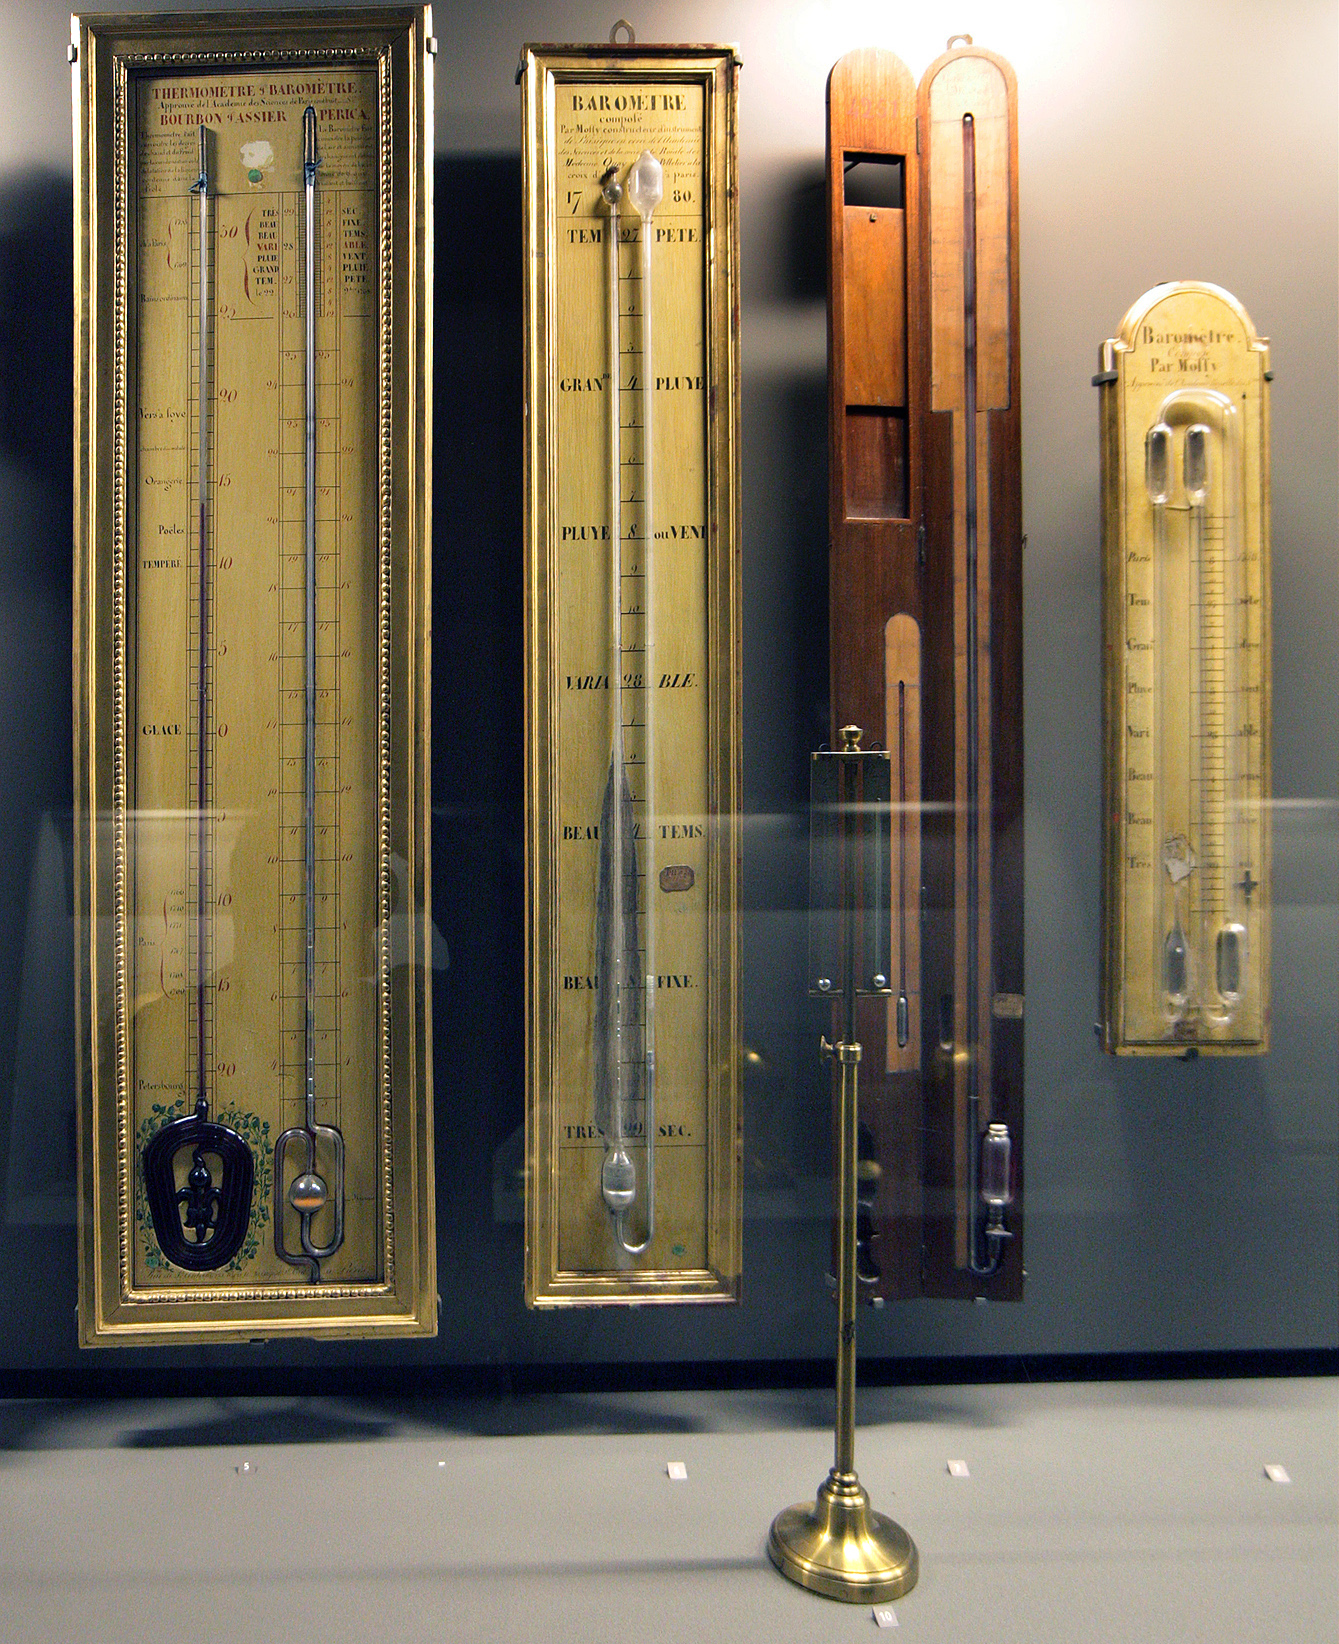
\includegraphics[width=0.33\textwidth]{Old-barometers.jpg}
    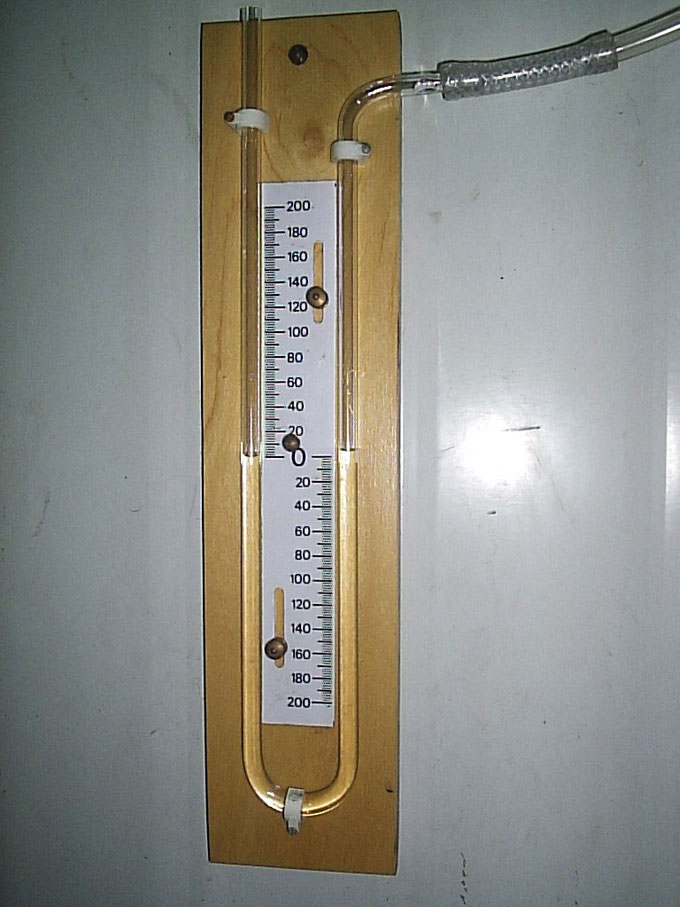
\includegraphics[width=0.33\textwidth]{Manometre.png}
    \caption[Baròmetre i Manòmetre diferencial]{El baròmetre (esquerra) utilitza una columna de mercuri per determinar la pressió atmosfèrica. Un manòmetre diferencial (dreta) mesura la diferència entre les pressions externes i d'un determinat gas.}
    \label{fig:Manometre}
    \end{figure}

La pressió és definida com la força per unitat d'àrea que un gas exerceix sobre les parets del recipient que el conté. S'expressa comunament en unitats com pascals (\si\pascal) o atmosferes (\si\atm). Matemàticament:
\begin{equation}
\text{Pressió} = \frac{\text{Força}}{\text{Àrea}} = \frac{\text{massa} \times \text{acceleració}}{\text{Àrea}} = \frac{\text{massa} \times \text{acceleració}}{\text{Volum / alçada}} 
\end{equation}
Per tant, la pressió es calcula com:
\begin{equation}
P = \rho \cdot g \cdot h,
\end{equation}
on $\rho$ és la densitat, $g$ l'acceleració gravitatòria i $h$ l'alçada.

Calculem ara què és una atmosfera quan s'expressa en funció de força per àrea unitaria. Considerem una columna de mercuri amb una alçada de 760 mm. Sabem que la densitat del mercuri és $13.6 \cdot 10^3 \si{\kg\per\meter\tothe{3}}$ i l'acceleració gravitatòria és $9.8 \si{\meter\per\square\second}$.  Considerem un tub baromètric la superfície de secció transversal del qual és 1 \si{\square\cm}. Aleshores, la força que exerceix la columna de mercuri sobre aquesta superfície és igual a la massa del mercuri que es troba al tub, multiplicada per l'acceleració deguda a la gravetat. A la vegada, la massa del mercuri que està en el tub és el volum del mercuri multiplicat per la seva densitat a $0^{\circ}\text{C}$. Així doncs, es té:

\[
\text{força} = 
\]
\[
= \text{densitat del Hg} \times \text{alçada} \times \text{àrea} \times \text{acceleració}
\]
\[
= 13,59 \, \frac{\si\g}{\si{\cubic\cm}} \times 76,00 \, \si{\cm} \times 1,000 \, \si{\square\cm} \times 980,7 \, \frac{\si{\cm}}{\si{\s}^2}
\]
\[
= 1,013 \times 10^6 \, \si\g \cdot \frac{\si\cm}{\si{\s}^2} = 10,13 \, \si\kg \cdot \frac{\si\m}{\si{\s^2}}
\]
\[
= 10,13 \si{\newton}.
\]

Aquesta és la força que exerceix una columna de mercuri de 760 mm d'alçada i d'1 $\text{cm}^2$ de superfície de secció transversal. Per tant, és també la força per unitat de superfície (un centímetre quadrat) que correspon a la pressió d'una atmosfera. Així, es té que:

\[
1 \, \si{\atm} = 760,0 \, \si\mmHg= 760 \,\si\torr
= 1,013 \times 10^6 \, \si{\dyn\per\square\cm} = 1,013 \times 10^5 \, \si{\newton\per\square\meter}.
\]

Els gasos es comporten segons certes lleis empíriques que han estat establertes experimentalment. Aquestes lleis condueixen finalment a la formulació de la llei dels gasos ideals.

\section{Llei de Boyle}
La llei de Boyle estableix que, a temperatura constant, la pressió \( P \) d'un gas és inversament proporcional al seu volum \( V \):
\begin{equation}
    P V = \text{constant}
\end{equation}
On \( P \) s'expressa en \si{Pa} (pascals) i \( V \) en \si{m^3}.

\section{Llei de Charles}
La llei de Charles afirma que, a pressió constant, el volum d'un gas és directament proporcional a la seva temperatura absoluta \( T \):
\begin{equation}
    \frac{V}{T} = \text{constant}
\end{equation}
On \( T \) es mesura en \si{K} (kelvins).

\section{Llei d'Amonton (o de Gay-Lussac)}
La llei de Gay-Lussac és una llei dels gasos que estableix que la pressió \( P \) exercida per un gas (d'una massa donada i mantingut a volum constant) varia directament amb la temperatura absoluta del gas:
\begin{equation}
    T \propto P \quad \text{o} \quad P = \text{constant} \times T
\end{equation}
En altres paraules, si un gas ideal està confinat en un recipient amb volum constant i s'incrementa la temperatura, la pressió augmentarà proporcionalment a la temperatura.


\section{Llei dels Gasos Ideals}
Combinant les tres lleis anteriors, obtenim la llei dels gasos ideals:
\begin{equation}
    P V = n R T
\end{equation}
On:
\begin{itemize}
    \item \( P \) és la pressió en \si{Pa}
    \item \( V \) és el volum en \si{m^3}
    \item \( n \) és el nombre de mols
    \item \( R \) és la constant dels gasos, amb valor \( \SI{8.314}{J.mol^{-1}.K^{-1}} \)
    \item \( T \) és la temperatura en \si{K}
\end{itemize}

\section{Llei de Dalton}
La llei de les pressions parcials de Dalton estableix que la pressió total d'una mescla de gasos ideals és igual a la suma de les pressions parcials dels gasos individuals en la mescla. Matemàticament, es pot expressar així:

\[
P_{\text{total}} = P_1 + P_2 + P_3 + \cdots + P_n
\]

on \(P_{\text{total}}\) és la pressió total de la mescla, i \(P_1, P_2, \dots, P_n\) són les pressions parcials dels diferents gasos presents a la mescla.

La pressió parcial d'un gas és la pressió que exerciria aquest gas si ocupés tot el volum per si sol, a la mateixa temperatura.


